% 经管类标准中文学术论文 LaTeX 模板
% ==========================================

\documentclass[a4paper, 12pt]{article}    % 英文文档类
\usepackage[english]{babel}% 英文断词、标题（Table/Figure）
% ==================== 宏包调用区 ====================
\usepackage[margin=1in]{geometry}    % 页面边距设置为 1 英寸（标准要求）
\usepackage{amsmath, amssymb}        % 数学公式宏包
\usepackage{graphicx}                % 插入图片宏包
\usepackage{booktabs}                % 三线表宏包（配合 Stata 的 esttab）
\usepackage{threeparttable}          % 表格底端加注释宏包（强烈推荐）
\usepackage{multirow}                % 表格合并单元格
\usepackage{makecell}                % 表格内换行
\usepackage{caption}
% 把“表”换成 Table，“图”换成 Figure
\renewcommand{\tablename}{Table}
\renewcommand{\figurename}{Figure}
\usepackage{setspace}                % 设置行距
\usepackage[colorlinks=true, linkcolor=blue, citecolor=blue, urlcolor=blue]{hyperref} % 超链接及交叉引用颜色
\usepackage[numbers, sort&compress]{natbib}

% 全局行距设置 (1.5倍行距适合盲审和阅读)
\setstretch{1.5}

% 图表标题格式设置
\captionsetup[table]{skip=5pt, font=bf} % 表格标题加粗，与表格距离 5pt
\captionsetup[figure]{skip=5pt, font=bf}
\usepackage{float}

\title{ VRP in the Chinese Market: An Empirical Analysis Based on CSI 300 ETF Options}
\author{
    Guiyuan Ma$^{1}$ \qquad Zhuangfei Ma$^{1}$% \qquad Xinfeng Ruan$^{1}$
    \\
    $^{1}$School of Economics and Finance, Xi'an Jiaotong University %\\
    %$^{2}$School of Economics, Another University
}

\date{}  % 清空日期

\begin{document}

\maketitle

	\begin{abstract}
		As a core forward-looking indicator for measuring market risk pricing and investor sentiment, the VRP has long been a central topic in the field of asset pricing due to its predictive power regarding asset returns. Based on 5-minute high-frequency return data for the Huatai-PineBridge CSI 300 ETF on the Shanghai Stock Exchange from January 2020 to October 2025, along with corresponding daily option trading data, this paper systematically examines the VRP’s predictive power for the CSI 300 ETF’s returns, its term structure characteristics, and its asymmetric effects. Additionally, the study introduces the Heterogeneous Autoregressive Realized Volatility (HAR-RV) model to optimize the construction of the VRP. The study found that: 1) VRP possesses significant predictive power for ETF returns and exhibits distinct term structure characteristics—it shows positive predictive power within the 30- to 90-day medium-term window, while reversing to negative in the 120-day and longer-term windows, with significance reaching the 1‰ level; 2) The predictive effects of positive and negative VRP exhibit significant asymmetry, and the predictive power of the downside volatility risk premium shows a marked decline in the 360-day ultra-long-term window; 3) The HAR-VRP indicator, constructed based on the HAR-RV model, outperforms the traditional VRP within a multiple regression framework; the goodness of fit improves across all forecast horizons of 60 days and longer, peaking around the 180-day horizon; 4) Implied volatility-related variables generally exhibit robust significance in long-term forecasts, confirming that forward-looking market expectations are the core driver of long-term return forecasts. This study deepens the empirical analysis of the VRP’s return forecasting effect in China’s ETF options market and provides insights for institutional investors regarding asset allocation, risk management, and the improvement of derivatives market regulations.
        \par\textbf{Keywords:} VRP; CSI 300 ETF; Return forecasting, HAR-RV model; Model-free implied volatility
	\end{abstract}

\newpage  % 可选：让目录单独占一页
%\tableofcontents
%\newpage  % 可选：让目录单独占一页

\section{Introduction}

As China’s capital market continues to deepen its reforms and expand its opening-up, the financial derivatives market is playing an increasingly vital role in price discovery, risk management, and asset allocation. In December 2019, the Shanghai Stock Exchange listed the Huatai-PineBridge CSI 300 ETF Options. As China’s first ETF options product covering broad-based indices in the Shanghai and Shenzhen markets, its launch filled a gap in risk management tools for core broad-based indices in the A-share market, becoming a key instrument for institutional and retail investors to hedge market risks and express market views. Since 2020, global markets have been impacted by multiple events, including the COVID-19 pandemic, shifts in the Federal Reserve’s monetary policy cycle, geopolitical conflicts, and fluctuations in the domestic economic cycle. Volatility in the A-share market has significantly intensified, and investor demand for hedging against tail risks and volatility pricing has continued to rise. The CSI 300 ETF options market has advanced significantly in trading activity, open interest, and pricing efficiency, providing high-quality market data and research scenarios for studies on volatility risk pricing and forecasting in China’s capital markets.

Volatility is a core variable in modern financial theory, permeating the entire process of asset pricing, portfolio construction, risk management, and derivatives pricing. Unlike historical volatility and realized volatility, which merely reflect past price fluctuations, the Volatility Risk Premium (VRP)—defined as the difference between implied volatility under a risk-neutral measure and realized volatility under an actual measure—directly reflects the risk compensation that market investors are willing to pay to hedge against future volatility risk. It serves as a core forward-looking indicator of market risk appetite, investor sentiment, and expectations of future returns. VRP has become a central research focus in the disciplines of asset return forecasting and volatility pricing across global capital markets since the classic research conducted by Bollerslev and others confirmed that VRP possesses significant predictive power for stock market returns.

Based on existing research, studies on the VRP in mature overseas markets have established a relatively comprehensive theoretical system and empirical framework, generally confirming that the VRP possesses significant medium- to long-term predictive power for stock market returns and exhibits a significant asymmetric effect in the pricing of upward and downward volatility. Domestic research on this topic remains in a phase of ongoing development. Existing studies primarily focus on spot indices such as the Shanghai Composite Index and the CSI 300 Index, or concentrate on the Shanghai 50 ETF options market; research utilizing long-term, high-frequency data following the listing of CSI 300 ETF options remains relatively scarce. At the same time, existing studies differ in their conclusions regarding the direction and significance of VRP across different forecast horizons. There has been insufficient exploration of the asymmetric predictive effects of positive and negative VRP in China’s markets, and few studies have optimized the construction of VRP through volatility forecasting models to enhance its predictive performance for asset returns. Furthermore, since China’s official volatility index (iVIX) ceased publication in 2018, constructing model-free implied volatility based on high-frequency trading data from the options market to derive a VRP indicator tailored to the characteristics of the Chinese market holds significant theoretical and practical value.

Based on this, this paper selects 5-minute high-frequency return data for the Huatai-PineBridge CSI 300 ETF on the Shanghai Stock Exchange from January 2020 to October 2025, as well as corresponding daily trading data for CSI 300 ETF options, as the research sample, to systematically investigate the predictive power, term structure, and asymmetry effects of the VRP on the returns of the CSI 300 ETF. Furthermore, the paper optimizes the VRP construction method based on the Heterogeneous Autoregressive Realized Volatility (HAR-RV) model to further enhance its predictive performance for asset returns.

The research in this paper is primarily divided into four sections: First, based on model-free implied volatility methods and 5-minute high-frequency data, we construct full-sample VRP, positive VRP, and negative VRP indicators, respectively. At the same time, we select relevant indicators such as the mean of implied volatility, call and put option trading volumes, the implied volatility spread, and the VIX index as control variables, clearly defining the core variables and their calculation methods; Second, univariate and multivariate benchmark regression models are constructed, employing HC3 White robust standard errors to address heteroskedasticity issues; systematically testing the VRP’s forecasting ability, direction of impact, and term structure characteristics for the CSI 300 ETF return across eight forecast horizons (1-day, 7-day, 30-day, 60-day, 90-day, 120-day, 180-day, and 360-day), while comparing the asymmetric forecasting effects of positive and negative VRPs; Third, we introduce the HAR-RV model to construct a volatility forecasting model based on realized volatility across daily, weekly, and monthly time scales. By substituting historical realized volatility with model-predicted realized volatility, we develop an optimized HAR-VRP indicator to test its forecasting ability for returns and compare its fit with that of the benchmark model; Fourth, based on the empirical results, we summarize the research conclusions to provide empirical evidence and recommendations for institutional investors’ asset allocation, risk management, and option strategy development, as well as for regulatory authorities in improving the institutional framework of the derivatives market.

The research contributions of this paper are primarily reflected in three aspects: First, the sample is highly timely and targeted. The research sample covers the entire operational cycle from 2020 to 2025 following the listing of CSI 300 ETF options, encompassing multiple rounds of extreme market conditions such as the impact of the pandemic and market transitions between bull and bear markets. Compared to existing studies, the conclusions are more aligned with the current development status of China’s ETF options market and possess greater robustness and practical reference value; Second, the study deepens research on the asymmetric effects of VRP forecasting capabilities in China’s market. By decomposing positive and negative VRPs, it systematically examines the differentiated impacts of upward and downward volatility risk premiums on returns across various time horizons, thereby supplementing empirical evidence regarding asymmetric volatility pricing in emerging markets; Third, the study achieves marginal innovation in methodology by integrating the HAR-RV volatility forecasting model with the construction of the VRP indicator. By optimizing the calculation method for realized volatility, it improves the predictive performance of VRP and demonstrates that HAR-VRP offers superior fitting performance compared to traditional VRP in medium- to long-term yield forecasting, thereby providing new insights and methodologies for research on asset yield forecasting and volatility pricing.

\section{Literature}

\subsection{Research on the Definition and Measurement of VRP}

The VRP is a core concept in asset pricing. Essentially, it represents the risk compensation that market investors are willing to pay to hedge against the volatility risk associated with future uncertainty. Quantitatively, it is defined as the difference between an asset’s implied volatility and its realized volatility and serves as a key indicator for measuring the market’s pricing of volatility risk. From an economic perspective, the VRP is typically positive, representing the premium investors are willing to pay to avoid future volatility risk. Its magnitude directly reflects the market’s overall risk aversion and the level at which uncertainty is priced in; only when extreme tail-risk events occur in the market or when investors’ expectations regarding future volatility exhibit systematic biases does VRP temporarily turn negative. This characteristic also makes it a crucial leading indicator for monitoring extreme market sentiment and risk conditions.

Regarding the theoretical origins of the VRP, Merton (1973) first explicitly stated in the Intertemporal Capital Asset Pricing Model (ICAPM) that the expected return on an asset depends not only on the risk-return profile of the market portfolio but also on the volatility risk of the set of future investment opportunities, thereby providing the core theoretical foundation for the systematic pricing of volatility risk. Subsequent classic research by Bollerslev et al. (2009) further clarified the economic implications of the VRP, defining it as the difference between risk-neutral expected volatility and realized volatility in the real world. This definition directly reflects the market’s willingness to price future volatility risk and has since become the core consensus in subsequent academic research on the VRP. Concurrently, this study rigorously demonstrated the intrinsic link between the VRP and investor marginal utility through a stochastic discount factor framework, establishing the VRP’s role as a systemic risk factor in asset pricing. This approach fundamentally shifted the perspective from early research—where volatility was treated merely as an auxiliary variable for returns—and integrated it into the core analytical framework of asset pricing. Subsequent research, building upon this core definition, distinguished the measurement boundaries between the VRP and the Variance Risk Premium (VRP). Among these, the pricing measure based on the first-order moment of volatility has become the mainstream analytical paradigm for VRP in academia, providing a unified academic standard for the definition of core variables in this paper.

Regarding the measurement methods of the VRP, the academic community has established a mainstream measurement framework centered on the “implied volatility minus realized volatility” approach. Regarding the measurement of implied volatility, Britten-Jones and Neuberger (2000) first proposed the model-free implied volatility method. This method breaks free from the parameter constraints of traditional option pricing models and can more accurately extract the market’s unbiased expectations of future volatility through option prices at different strike prices. It is now widely used in the compilation of volatility indices and academic research across major global capital markets, becoming the mainstream method for measuring implied volatility. Compared to implied volatility derived from the Black-Scholes option pricing model framework, model-free implied volatility does not require strict assumptions about the return distribution of the underlying asset. It effectively avoids measurement errors caused by model specification biases while fully utilizing information from out-of-the-money and in-the-money option prices at different strike prices to more comprehensively capture the market’s expectations of future volatility across the entire distribution. In response to the characteristics of China’s options market—such as short contract maturities and limited strike price coverage—domestic scholars have adapted and optimized this method for the local context. By employing interpolation and extrapolation techniques to refine the construction of the volatility surface, they have further improved the measurement accuracy of model-free implied volatility in the Chinese market, thereby providing localized methodological references for the estimation of variables in this paper. Regarding the measurement of realized volatility, the seminal work by Andersen and Bollerslev (1998) laid the foundation for high-frequency realized volatility estimation. Their research demonstrated that realized volatility constructed using high-frequency intraday data can more accurately capture the true volatility level of an asset, significantly outperforming traditional volatility measurement methods based on daily data. This method has also become the core paradigm for constructing realized volatility in current VRP calculations. Subsequent academic research has conducted extensive studies on optimizing the measurement of high-frequency realized volatility. To address issues such as microstructural noise in intraday high-frequency data and overnight gaps during non-trading hours, a series of robust correction methods—including noise reduction and overnight return adjustments—have been proposed, further enhancing the ability of realized volatility to characterize the true volatility levels of the underlying assets. Compared to volatility measures derived from GARCH-type models based on daily returns, high-frequency realized volatility offers the advantages of being model-free, parameter-free, and featuring higher fitting accuracy. It can more precisely align with the forward-looking horizon of option implied volatility, making it the optimal proxy for realized volatility in VRP estimation. The aforementioned measurement framework also provides the core methodological basis for the VRP estimation of the CSI 300 ETF discussed in this paper.

\subsection{Research on the Predictive Effect of VRP on Asset Returns}
The predictive power of the VRP for asset returns is a central research focus in the field of asset pricing and constitutes the core theme of this study. Existing mainstream research generally confirms that the VRP possesses significant predictive power for asset returns and serves as an important systematic risk factor driving expected returns.

In relevant studies of mature international markets, the academic community has established a relatively well-developed research framework and set of conclusions. Bollerslev et al. (2009), based on research in the U.S. stock market, were the first to confirm that market-level VRP possesses significant positive predictive power for the future returns of the S&P 500 Index, with this predictive power being most pronounced in the short to medium term, such as on a monthly or quarterly basis. The study also noted that VRP essentially reflects the market’s overall level of risk aversion. When VRP rises, it indicates that market investors demand higher risk compensation for volatility risk, which in turn pushes up the future expected returns of assets, providing a core economic explanation for the return-predicting effect of VRP. This core conclusion completely overturns the pricing logic under the traditional CAPM framework, which focuses solely on return-risk relationships, and confirms that volatility risk itself is an independent pricing factor driving expected asset returns. Subsequent extension studies by Bollerslev et al. (2014) further decomposed the structure of the VRP, distinguishing it into risk premiums derived from “good volatility” (volatility associated with positive returns) and “bad volatility” (volatility associated with negative returns). They found that the risk premium corresponding to bad volatility possesses significantly stronger predictive power for future asset returns, thereby deepening the academic community’s understanding of the intrinsic structure of the VRP’s predictive effect. Building on this foundation, numerous scholars have conducted further theoretical extensions and empirical validations. Drechsler and Yaron (2011), based on a long-term risk model, theoretically demonstrated that the VRP incorporates market pricing information regarding macroeconomic uncertainty and tail risks, thereby enabling effective forecasting of future asset returns. The study also found that the VRP possesses significant forward-looking predictive power regarding macroeconomic growth; its predictive effect on asset returns essentially represents the advance pricing of expectations regarding macroeconomic fundamentals, thereby providing theoretical support at the macroeconomic level for the VRP’s return forecasting capability. Rapach et al. (2013), in a cross-country study of multiple mature capital markets worldwide, further found that the VRP’s ability to predict stock market returns is universally present across global markets, making it a globally priced factor with cross-market robustness. At the same time, the study also found that the VRP in the U.S. market exhibits a significant cross-border spillover effect on stock returns in other global capital markets, confirming the VRP’s role as a globally priced systemic risk factor. Of course, there are also some heterogeneous research findings in the academic community. For instance, some scholars have found that the predictive power of VRP significantly declines over ultra-long-term forecasting horizons (more than one year), and its predictive efficacy also weakens temporarily during extreme crisis periods marked by liquidity shortages. These heterogeneous findings also provide a literature reference for this paper’s analysis of heterogeneity in forecasting horizons and market environments. The aforementioned classic studies provide the core theoretical foundation and empirical framework for this paper’s examination of VRP’s return forecasting for the CSI 300 ETF.

\subsection{A Study on the Localization of VRP in China’s Capital Markets}

With the continuous improvement of China’s capital market derivatives system, particularly following the official launch of CSI 300 ETF options in 2019, research on the Volatility Risk Premium (VRP) for core broad-market indices in China’s A-share market has gradually become a hot topic in academic circles. Existing studies have preliminarily validated the pricing properties and return forecasting effects of the VRP for CSI 300-related indices.

At the level of early foundational research, domestic scholars have conducted a significant amount of pioneering work on volatility risk pricing in China’s stock market. Chen Rong and Zheng Zhenlong (2009) were the first to undertake systematic model-building and empirical testing of the VRP in China’s stock market, confirming that the volatility risk in the A-share market exhibits a significant pricing effect and laying a core theoretical foundation for subsequent localized research. Subsequent research by Zheng Zhenlong and Liu Yangshu (2013) further expanded upon these findings. Their study revealed that the index VRP in China’s A-share market possesses significant predictive power regarding future market index returns, and this predictive power remains significant even after controlling for traditional Fama-French three-factor models such as size, value, and momentum, thereby confirming the independent pricing capability of VRP in China’s stock market. Research by Chen Guojin et al. (2018), adopting a tail-risk-pricing perspective, confirmed that the VRP in China’s A-share market incorporates pricing information regarding extreme tail risks. Its predictive power for market returns is particularly pronounced during tail-risk events, further enriching the pricing implications of VRP in China’s emerging capital markets. At the same time, early research also examined the institutional characteristics of China’s options market during its early development phase, verifying the applicability of VRP in the Chinese market under different measurement methods, thereby laying a methodological foundation for subsequent refined studies following the formal launch of the derivatives market.

Regarding targeted research on the CSI 300 ETF and its corresponding options market, the listing of CSI 300 ETF options has provided the academic community with high-quality exchange-traded options data for conducting detailed empirical research. Based on simulated trading data for stock index options, Huang Yizhou and Zheng Zhenlong (2016) validated the applicability of model-free implied volatility in China’s market, confirming that it can capture market volatility expectations more accurately than traditional methods. Chen Rong et al. (2021), using real trading data from the CSI 300 ETF options market following its launch, systematically measured the VRP in China’s CSI 300 ETF market for the first time. They confirmed the existence and time-varying nature of the VRP in this market and found that it contains rich information on market risk and investor sentiment. Subsequent research further revealed that the listing of CSI 300 ETF options significantly enhanced the volatility pricing efficiency of China’s A-share market, resulting in a marked improvement in the predictive power of the VRP—constructed using these option data—for the returns of the underlying assets compared to the simulation trading phase. At the same time, some scholars have conducted preliminary analyses of the differences in VRP between the CSI 300 ETF and the CSI 300 Index, finding that not only does the ETF's VRP incorporate macro-level pricing information for volatility risk from the index but it also integrates microstructural information such as on-exchange trading premiums or discounts, capital flows, and liquidity premiums. Consequently, it possesses stronger marginal explanatory power and predictive value for the future returns of the underlying ETF. Furthermore, numerous subsequent studies have further pointed out that, as the largest and most liquid broad-market ETF product in the A-share market, the CSI 300 ETF’s VRP more directly reflects the risk-pricing preferences of on-exchange investors. Compared to index-level VRP, it offers stronger practical explanatory power and predictive value for the returns of tradable securities. Existing research has also developed corresponding market timing and hedging strategies based on the VRP of the CSI 300 ETF, confirming that investment strategies built on VRP signals can significantly enhance the investment returns of the CSI 300 ETF and effectively control downside risk. This highlights the practical value of VRP in ETF investment practice and provides a real-world application basis for the research in this paper.

\subsection{Literature Review}

Based on a comprehensive review of existing research, the academic community has established a systematic body of work regarding the definition, measurement methods, and return forecasting effects of VRP. The core consensus is that VRP is a key systematic factor reflecting the pricing of market volatility risk, and it possesses significant predictive power for the returns of major asset classes—including equities, bonds, foreign exchange, and commodity futures—in mature global capital markets; simultaneously, localized research on China’s capital markets has validated VRP’s pricing attributes and return forecasting effects in both the stock market (CSI 300-related securities) and the commodity futures market, laying a solid theoretical and empirical foundation for subsequent research.

However, existing research still has gaps that require further exploration, which serve as the core research entry points for this paper. All research gaps are strictly defined within the scope of this paper’s study of the CSI 300 ETF as a single instrument and do not exceed the actual research boundaries of this paper:

First, existing domestic research on the return forecasting effects of VRP generally follows two main lines of inquiry: one focuses on return forecasting for the CSI 300 price index, while the other is scattered across pricing studies of other derivative categories such as commodity futures. Detailed, targeted return forecasting research on the CSI 300 ETF—a core broad-market product directly tradable on China’s A-share market—remains to be deepened. Most existing studies take the CSI 300 price index—which is not directly tradable—as their core research object. However, the CSI 300 ETF differs fundamentally from the price index in terms of trading mechanisms, return structures, investor composition, and trading frictions. Consequently, the conclusions drawn from existing studies on the index cannot be directly applied to the actually tradable ETF product. There remains significant room for supplementary research specifically focused on the CSI 300 ETF.

Second, most existing domestic research on CSI 300-related instruments has focused on verifying the existence of the Value-at-Risk (VRP) and analyzing its pricing attributes, while in-depth empirical tests of the predictive efficacy of VRP on CSI 300 ETF returns remain relatively insufficient. Most existing studies have merely verified the existence of the predictive effect, failing to fully clarify the differences in VRP’s predictive performance for CSI 300 ETF returns across different forecast horizons. Furthermore, they have not conducted systematic, multi-dimensional tests on the robustness of the predictive results. The depth of such research remains to be expanded, and this constitutes the core empirical research content of this paper.

Third, most existing studies treat VRP pricing research in the stock market and the commodity futures market as separate topics. Few studies have conducted theoretical comparisons between the well-established conclusions regarding VRP in the commodity futures market and the predictive effects observed in the CSI 300 ETF market, failing to fully clarify the similarities and differences in VRP pricing logic between broad-based ETFs and commodity futures. Furthermore, analysis of the intrinsic transmission mechanisms through which VRP influences the returns of the CSI 300 ETF remains relatively scarce. Most studies have remained at the level of verifying predictive effects, failing to deeply dissect the underlying risk-pricing transmission logic; this also represents an important area for further research in this paper.


	% --- 3. 研究设计 ---
\section{Research Design}

	\subsection{Sample Selection}
	This paper uses 5-minute return data for the Huatai-PineBridge CSI 300 ETF, listed on the Shanghai Stock Exchange from January 2020 to October 2025, and conducts a follow-up study using daily data for the Huatai-PineBridge CSI 300 ETF options.
	The 5-minute-level data for the CSI 300 ETF used in this paper was obtained from the JoinQuant platform, while the relevant option data was sourced from the Wind database. Data cleaning and empirical regression were performed in a Python environment.
    

\subsection{Model Building}
\subsubsection{Realized Volatility}
Realized volatility is calculated using high-frequency returns over a given period. To some extent, realized volatility shares the same characteristics and significance as historical volatility; the key difference is that realized volatility can be derived by aggregating higher-frequency data when historical volatility is unavailable for short time horizons. In this paper, realized volatility is calculated as follows:

        \begin{equation}
        RV_t = 100\sqrt{252\sum_{i=1}^{M} r_{t,i}^2}, \quad r_{t,i} = \ln P_{t,i} - \ln P_{t,i-1}
        \end{equation}
        
To ensure that the calculated realized volatility is of roughly the same order of magnitude as the implied volatility, the formula for calculating realized volatility in this paper has been modified as shown above. Meanwhile, the positive and negative components of realized volatility are as follows:

        \begin{equation}
        RV^+_t = 100\sqrt{252\sum_{i=1}^{M} r_{t,i}^2I_{[r_{t,i} > 0]}}, \quad r_{t,i} = \ln P_{t,i} - \ln P_{t,i-1}
        \end{equation}
        \begin{equation}
        RV^-_t = 100\sqrt{252\sum_{i=1}^{M} r_{t,i}^2I_{[r_{t,i} < 0]}}, \quad r_{t,i} = \ln P_{t,i} - \ln P_{t,i-1}
        \end{equation}
        
Using the methods described in the previous two equations, we can decompose the overall realized volatility into positive and negative components.

\subsubsection{Implied Volatility}
%隐含波动率的计算最早起源于BS模型（Black-Scholes Option Pricing Model）。在人们可以从市场得到期权价格的前提下，便可以通过BS模型反推出标的物的隐含波动率。
This paper uses the model-free implied volatility (MFIV) proposed by Britten-Jones et al. (2000) to calculate the VRP. The exact formula for the model-free implied volatility is given by the following equation:

\begin{equation}
    E_0^F \left[ \int_0^T \left( \frac{dF_t}{F_t} \right)^2 \right] = 2\int_0^\infty \frac{C^F(T, K) - \max(0, F_0 - K)}{K^2} dK
\end{equation}
In this equation, the left-hand side represents the variance under the risk-neutral measure, i.e., the implied variance; $C^F(T, K)$ denotes the price of a call option with a remaining maturity of T and a strike price of K; and $max(0, F_0 - K)$ denotes the option’s intrinsic value.
Although this equation provides a method for calculating IV without using the Black-Scholes model, actual market conditions do not support integration over a continuous range of strike prices (K) in the above equation. In practice, the calculation of model-free implied volatility is as follows:
\begin{equation}
    \sigma^2 = \frac{2}{T} \sum_i \frac{\Delta K_i}{K_i^2} e^{RT} Q(K_i) - \frac{1}{T} \left[ \frac{F}{K_0} - 1 \right]^2
\end{equation}

Here, $K_i$ is the strike price of the $i$th option, $\Delta K_i$ is the difference between the strike prices of adjacent options, defined as $\frac{K_{i+1}-K_{i-1}}{2}$, T is the option expiration time, and F is the forward price at expiration. $K_0$ is the strike price of the at-the-money option, and $Q(K_i)$ represents the price of the out-of-the-money options with a strike price of $K_i$.

Similarly, the model-free positive implied variance can be calculated as follows:

\begin{equation}
    \sigma^2_+ = \frac{2}{T} \sum_i \frac{\Delta K_i}{K_i^2} e^{RT} C(K_i) - \frac{1}{T} \left[ \frac{F}{K_0} - 1 \right]^2
\end{equation}

Model-free negative implied variance:

\begin{equation}
    \sigma^2_- = \frac{2}{T} \sum_i \frac{\Delta K_i}{K_i^2} e^{RT} P(K_i) - \frac{1}{T} \left[ \frac{F}{K_0} - 1 \right]^2
\end{equation}

In addition, since the MFIV is relatively sensitive to changes in option expiration dates, this paper adopts the volatility index calculation method used by the Chicago Board Options Exchange (CBOE):

\begin{equation}
    VIX = 100\sqrt{\left( \frac{N_{T_1} - N_{30}}{N_{T_1} - N_{T_2}} \right) \sigma_1^2 + \left( \frac{N_{30} - N_{T_2}}{N_{T_1} - N_{T_2}} \right) \sigma_2^2}
\end{equation}

The Chinese market has consistently maintained a cautious stance toward the publication of the VIX index. After the China Volatility Index (iVIX) was first released in 2015, its publication through official channels was suspended in 2018. In this article, all VIX indices used are calculated based on the aforementioned process, using option trading data from the market.
	
    \subsection{Variables Defination}
        The dependent variable in this paper is the daily return of the Huatai-PineBridge CSI 300 ETF, and the independent variable is the VRP, which is calculated as follows:
        \begin{equation}
        VRP = IV - RV
        \end{equation}
        positive VRP:
        \begin{equation}
        VRP^+ = IV^+ - RV^+
        \end{equation}
        negative VRP:
        \begin{equation}
        VRP^- = IV^- - RV^-
        \end{equation}
        
        In the existing literature, the VRP has been shown to possess a certain predictive power for returns, with this predictive power being more pronounced over the long term. In this paper, while utilizing the VRP, we decompose it to explore its asymmetry in predicting asset returns.
        To reduce the model’s prediction error, this paper employs the control variables shown in Table \ref{variables}:
        
	\begin{table}[H]
		\centering
		\caption{Definition of Control Variables}
		\label{variables}
		\renewcommand{\arraystretch}{1.3} % 行高拉宽
		\begin{tabular}{llcp{7.5cm}}
			\toprule
			\textbf{Name} & \textbf{Symbol} & \textbf{Definition} \\
			\midrule
			Mean of Implied Volatility & $IV_{MEAN}$ & $\frac{1}{N}\sum_{i=1}^N BSIV_i$ \\
			Trading Volumes Spread Between Call and Put Option  & $VOLD$ & $VOL_{C}-VOL_{P}$ \\
			 IV Spread Between Call and Put Options & $IVD$ & $BSIV_{C}-BSIV_{P}$ \\
			    IV Spread Between Near-Term Call and Put Options & $IVDN$ & $BSIV_{C,NEAR}-BSIV_{P,NEAR}$ \\
			Negative Variance Risk Premium & $RIV$ & \textcolor{red}{$RV^2-IV^2$} \\
			 VIX Index & $VIX$ & $\sqrt{\dfrac{2}{T}\sum\limits_{i}\Delta K_i \cdot \dfrac{e^{rT}P(K_i)}{K_i^2}}$ \\
			 Positive VIX & $VIX^+$ & $\sqrt{\displaystyle\frac{2}{T}\sum\limits_{i}\frac{\Delta K_i}{K_i^2}e^{rT}C(K_i)}$ \\
		Negative VIX & $VIX^-$ & $\sqrt{\displaystyle\frac{2}{T}\sum\limits_{i}\frac{\Delta K_i}{K_i^2}e^{rT}P(K_i)}$ \\
			\bottomrule
		\end{tabular}
	\end{table}


    
\section{Empirical Analysis}
\subsection{Descriptive Statistics}
This section presents a descriptive statistical analysis of the main variables considered in the paper; the results are shown in Table \ref{描述性统计}. It can be observed that for any type of VRP, the minimum value is far below zero, indicating that the VRP exhibits excessively extreme values in the negative direction. In contrast, the VIX does not exhibit such exaggerated extremes or volatility levels, suggesting that realized volatility (RV) plays a decisive role in determining these extremes. This also indicates that China’s stock market is more active than its options market, making it more likely to experience extreme market conditions and to exhibit greater extremes.


In addition, Figure \ref{fig:placeholder} shows the correlation coefficients between the variables. As can be seen, IVD and IVDN, as well as VRP and RIV, exhibit high correlations due to their similar definitions. Similarly, VIX and the decomposed positive and negative VIX components, as well as VRP and the decomposed positive and negative VRP components, also show high correlations because their calculation processes are similar and they serve as components of the decomposition.

\begin{table}[htbp]
\centering
\footnotesize
\renewcommand{\arraystretch}{1.3} % 稍微压缩回归表的行距
\caption{Descriptive Statistics for Variables}
\label{描述性统计}
\begin{tabular}{lccccccccccc}
\toprule
& count & mean & std & min & 25\% & 50\% & 75\% & max \\
\midrule
$VRP^+$ & 1409 & 1.4869 & 6.8916 & -157.8062 & -0.1857 & 2.3530 & 4.5907 & 15.4973 \\
$VRP^-$ & 1409 & -2.0137 & 5.8377 & -69.7234 & -5.1510 & -1.0690 & 1.7763 & 10.0709 \\
$IV_{mean}$ & 1409 & 0.5237 & 0.2892 & 0.1074 & 0.3551 & 0.4514 & 0.6024 & 2.9412 \\
VRP & 1409 & 5.8368 & 5.2577 & -76.1787 & 3.9452 & 6.2886 & 8.3588 & 21.7916 \\
$VOLD$ & 1409 & 1.1346 & 0.6685 & 0.1084 & 0.6969 & 0.9937 & 1.3907 & 5.9516 \\
$IVD$ & 1409 & 1.7061 & 1.1647 & -0.3091 & 0.8182 & 1.5916 & 2.2285 & 6.1627 \\
$IVDN$ & 1409 & 0.9206 & 0.8415 & -0.0933 & 0.4103 & 0.7399 & 1.0923 & 4.6671 \\
VIX & 1409 & 19.7528 & 4.4300 & 12.9343 & 16.6058 & 18.8994 & 21.8143 & 44.5193 \\
RIV & 1409 & -1.6909 & 4.3510 & -10.2342 & -2.5748 & -1.8275 & -1.2012 & 125.8604 \\
$VIX^-$ & 1409 & 8.3732 & 4.7792 & 0.0001 & 5.6439 & 8.8168 & 11.3495 & 28.4079 \\
$VIX^+$ & 1409 & 12.2871 & 3.6245 & 2.4527 & 9.8070 & 11.7086 & 13.8196 & 31.0594 \\
\bottomrule
\end{tabular}
\end{table}

\begin{figure}
    \centering
    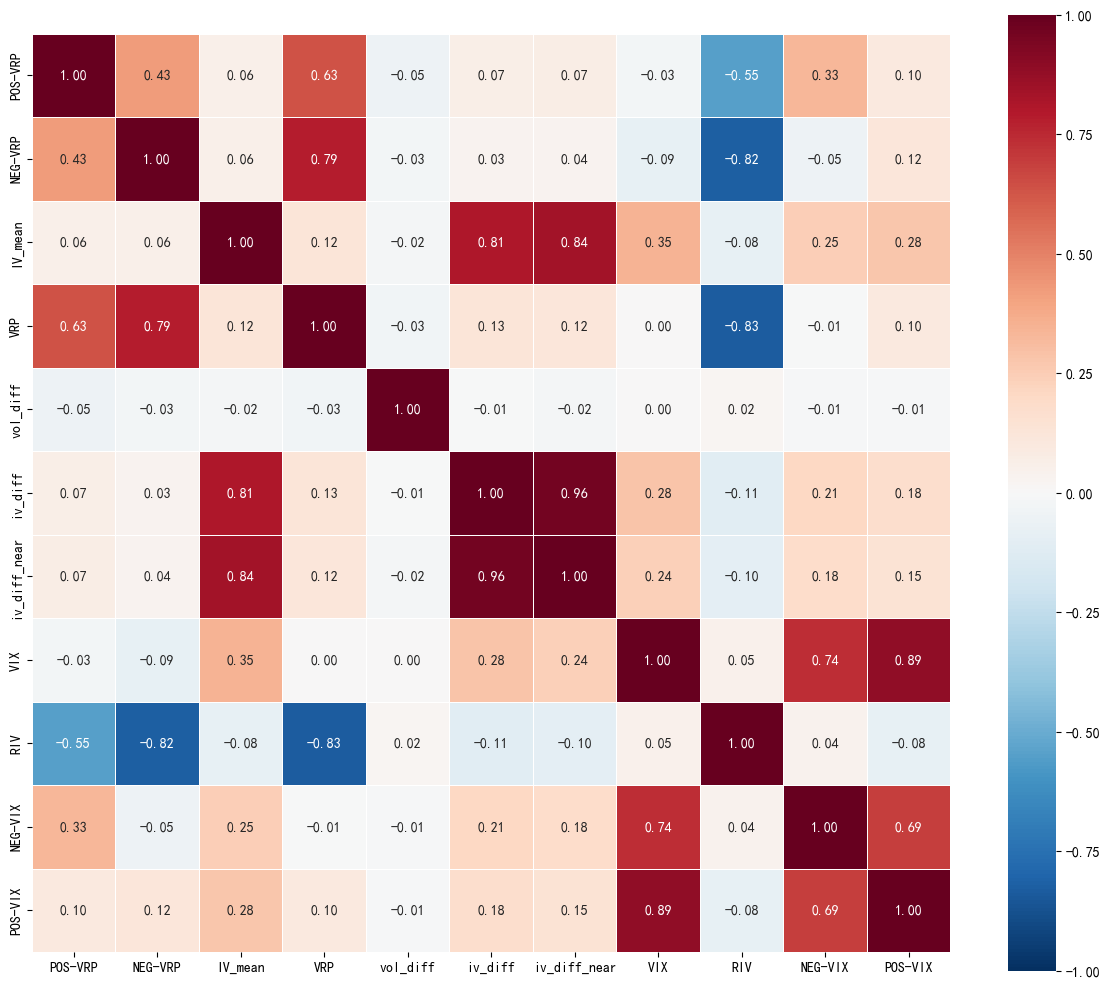
\includegraphics[width=0.8\linewidth]{correlation.png}
    \caption{Enter Caption}
    \label{fig:placeholder}
\end{figure}

\subsection{Empirical Analysis of a Univariate Benchmark Model}
        To examine the predictive power of the VRP on asset returns, this paper first employs a cross-period univariate regression as the baseline regression model. The baseline regression model is as follows:
        \begin{equation} \label{base}
		return_{t,t+h} = \alpha_0 + \alpha_i variable_{i,t} + \varepsilon_{t,t+h}
	\end{equation}
    
            Here, $return_{t,t+h}$ represents the return on the asset from time $t$ to time $t+h$, $variable_{i,t}$ represents the various variables at time $t$, including the VRP and other control variables, and $\varepsilon_{t,t+h}$ is the error term.
            Given that time series data in the financial sector typically exhibit heteroskedasticity, this paper uniformly employs HC3-type White heteroskedasticity-robust standard errors. This method accommodates any form of heteroskedasticity in regression analysis without altering the coefficients of ordinary least squares regression; instead, it only corrects the standard errors of the parameters, thereby making significance testing more effective.
            
        Table \ref{result1} presents the results of the benchmark regression, with predicted returns over horizons of 1, 7, 30, 60, 90, 120, 180, and 360 days. Based on the data in the table, it can be observed that the regression coefficients for VRP are close to zero for horizons of 7 days or less, and their significance levels are also low, indicating that VRP has virtually no predictive power for asset returns within a 7-day horizon. Over slightly longer horizons of 30 to 90 days, VRP begins to exhibit positive predictive power for returns, consistently maintaining a significance level of 5\% or higher. Over long horizons of 120 days or more, VRP demonstrates a significant and stable negative predictive power for returns at the 1‰ level. The decomposed $VRP^+$ and $VRP^-$ exhibit slightly weaker predictive power: they show no significance at any level for forecast horizons of 90 days or less; they are significant at the 0.1\% level for 120-day and 180-day horizons; but their significance declines again at the 360-day horizon.
        Regarding the remaining control variables, $IV_{MEAN}$ exhibits significance at the 1\% level for the 60-day forecast and maintains significance at the 1‰ level for long-term forecasts of 120 days or more. $VOL_{DIFF}$ demonstrates some predictive power only for the 60-day and 90-day horizons, which disappears as the forecast horizon extends. $IV_{DIFF}$ and $IV_{DIFF,NEAR}$ are defined similarly; apart from the fact that $IV_{DIFF,NEAR}$ is not significant at the 180-day horizon, the two exhibit similar performance across all other time periods. Although $RIV$ demonstrates some predictive power at the 7-day horizon, it only yields stable results in the long term. $VIX$, $VIX^+$, and $VIX^-$ exhibit similar behavior; all three begin to demonstrate some predictive power at the 30-day horizon and stabilize after 180 days.
        Based on the results of univariate regression, variables related to implied volatility all demonstrate consistent significance in long-term forecasting, whereas $VOL_{DIFF}$, which is based on trading volume, does not exhibit this phenomenon. Furthermore, among a series of variables related to implied volatility, VRP performs best across all time horizons. This suggests that VRP possesses superior predictive power for returns by combining information from both IV and RV.


      
\begin{table}[htbp]
\centering
\footnotesize % 缩小字号，防止表格过长跑出页面
\caption{Results of the univariate baseline regression model}
\label{result1}
\renewcommand{\arraystretch}{1.3} % 稍微压缩回归表的行距
\begin{tabular}{lcccccccc}
\toprule
&\multicolumn{8}{c}{Number of days of forecast lag: h}\\
\cmidrule(lr){2-9}
& 1    & 7    & 30   &  60  & 90   & 120  & 180  & 360 \\
\midrule
$VRP$ &0.0001 & 0 & 0.0011$^{**}$ & 0.0014$^{***}$ & 0.0014$^{*}$ & -0.0021$^{***}$ & -0.0053$^{***}$ & -0.0061$^{***}$  \\
&(0.197) & (-0.166) & (2.918) & (3.312) & (2.492) & (-4.342) & (-6.891) & (-4.920) \\
$VRP^+$ &-0.0002 & -0.0001 & 0.0003 & 0.0007 & 0.0006 & -0.0014$^{***}$ & -0.0026$^{***}$ & -0.0029$^{*}$  \\
&(-1.231) & (-0.551) & (1.094) & (1.820) & (1.190) & (-4.061) & (-3.949) & (-2.408) \\
$VRP^-$ &0.0001 & -0.0002 & 0.0005 & 0.0004 & 0.0009$^{*}$ & -0.0020$^{***}$ & -0.0027$^{***}$ & -0.0006  \\
&(0.796) & (-1.231) & (1.690) & (0.880) & (2.044) & (-4.346) & (-4.131) & (-0.646) \\
$IV_{MEAN}$ &-0.0012 & 0.0056 & -0.0116 & 0.0202$^{**}$ & -0.0135 & -0.0416$^{***}$ & -0.1238$^{***}$ & -0.1465$^{***}$  \\
&(-1.041) & (1.509) & (-1.950) & (2.612) & (-1.810) & (-4.552) & (-9.235) & (-8.170) \\
$VOLD$ &0.0008 & 0.0005 & -0.0035 & -0.0096$^{**}$ & -0.0103$^{**}$ & -0.0050 & -0.0018 & 0.0025  \\
&(1.645) & (0.453) & (-1.393) & (-2.705) & (-2.852) & (-1.200) & (-0.322) & (0.325) \\
$IVD$ &-0.0005 & -0.0006 & -0.0053$^{**}$ & -0.0051$^{*}$ & -0.0169$^{***}$ & -0.0250$^{***}$ & -0.0398$^{***}$ & -0.0419$^{***}$  \\
&(-1.555) & (-0.729) & (-3.216) & (-2.022) & (-6.323) & (-8.423) & (-11.586) & (-8.524) \\
$IVDN$ & -0.0006& -0.0001 & -0.0044$^{*}$ & -0.0038 & -0.0148$^{***}$ & -0.0222$^{***}$ & -0.0357$^{***}$ & -0.0320$^{***}$ \\
&(-1.417) & (-0.084) & (-2.134) & (-1.183) & (-4.540) & (-6.316) & (-9.136) & (-5.767) \\
$RIV$ &-0.0003 & 0.0003$^{**}$ & -0.0006 & -0.0011 & -0.0007 & 0.0023 & 0.0142$^{***}$ & 0.0149$^{***}$  \\
&(-0.323) & (2.703) & (-0.577) & (-0.800) & (-0.536) & (1.575) & (6.490) & (4.718) \\
$VIX$ &0 & 0.0001 & 0.0013$^{***}$ & 0.0013$^{*}$ & 0.0028$^{***}$ & 0 & -0.0135$^{***}$ & -0.0112$^{***}$  \\
&(0.333) & (0.682) & (3.576) & (2.107) & (6.954) & (-0.060) & (-11.932) & (-12.302) \\
$VIX^+$ &0.0001 & -0.0001 & 0.0013$^{**}$ & 0.0015$^{*}$ & 0.0039$^{***}$ & 0.0001 & -0.0142$^{***}$ & -0.0108$^{***}$  \\
&(0.935) & (-0.390) & (2.920) & (2.133) & (7.346) & (0.130) & (-11.173) & (-9.188) \\
$VIX^-$ &0.0001 & 0 & 0.0010$^{**}$ & 0.0005 & 0.0014$^{**}$ & -0.0009 & -0.0087$^{***}$ & -0.0043$^{***}$  \\
&(0.660) & (-0.004) & (2.775) & (0.963) & (2.900) & (-1.438) & (-11.843) & (-3.472) \\
\bottomrule
\multicolumn{9}{l}{\footnotesize \sym{*} \(p<0.05\), \sym{**} \(p<0.01\), \sym{***} \(p<0.001\)，The same applies below}\\
\end{tabular}
\end{table}

\subsection{Empirical Analysis of a Multivariate Benchmark Model}
To examine the interaction effects of variables on yield forecasts, this section employs a cross-period multiple regression model. The baseline model is as follows:
        \begin{equation}
		return_{t,t+h} = \alpha_0 + \alpha_1 VRP_t + \sum\alpha_i Control_{i,t} + \varepsilon_{t,t+h}
	\end{equation}
    
Here, $return_{t,t+h}$ represents the return on the asset from time $t$ to time $t+h$, $VRP$ is the VRP at time $t$, $Control_{i,t}$ denotes various control variables, and $\varepsilon_{t,t+h}$ is the error term.
Given the potential for multicollinearity among the variables, this section relies on the correlation matrix presented earlier in the text and retains only VRP, $IV_{MEAN}$, $VOL_{DIFF}$, $IV_{DIFF}$, and VIX as variables for the multiple regression analysis.

Table \ref{tab:univariate_baseline_rotated} presents the results of the multiple regression analysis. As shown in the table, VRP remains statistically significant at the 1\% level for forecast horizons of 30 days or longer, and reaches the 0.1\% level of significance at 30-, 90-, and 180-day horizons. Furthermore, VRP exhibits positive predictive power for horizons ranging from 30 to 90 days, but turns negative for horizons of 120 days or longer, which aligns with the findings of some existing studies. Regarding the remaining control variables, $IV_{MEAN}$ exhibits significant positive predictive power at the short-term 7-day level and the medium-to-long-term 60- to 120-day levels, but fails to hold at the long-term level. $IV_{DIFF}$ demonstrates significant negative predictive power at the 1\‰ level starting from the 7-day horizon. This indicates that various indicators derived from option implied volatility possess some predictive power for the underlying asset’s return to varying degrees and across different time horizons.
Furthermore, the model’s adjusted $R^2$ increases as the forecast horizon lengthens, reaching a maximum at 180 days before beginning to decline. This further illustrates that while VRP consistently exhibits significant predictive power in the long term, its predictive ability regarding the underlying asset’s return peaks around the six-month horizon.

\begin{table}[htbp]
\centering
\footnotesize
\caption{Results of the Multiple Regression Model}
\label{tab:univariate_baseline_rotated}
\renewcommand{\arraystretch}{1.3}
\begin{tabular}{lcccccccc}
\toprule
 & \multicolumn{8}{c}{Number of days of forecast lag: h} \\
\cmidrule(lr){2-9}
 & 1    & 7    & 30   & 60   & 90   & 120  & 180  & 360 \\
\midrule
$VRP$         & 0.0001 & -0.0001 & 0.0014$^{***}$ & 0.0011$^{**}$ & 0.0017$^{***}$ & -0.0015$^{**}$ & -0.0030$^{***}$ & -0.0029$^{**}$ \\
              & (0.266) & (-0.523) & (4.351) & (2.806) & (3.782) & (-3.094) & (-3.909) & (-2.613) \\
$IV_{mean}$   & 0.0004 & 0.0213$^{***}$ & 0.0055 & 0.0707$^{***}$ & 0.0629$^{***}$ & 0.0756$^{***}$ & 0.0055 & -0.0306 \\
              & (0.238) & (3.912) & (0.614) & (4.680) & (4.173) & (4.678) & (0.276) & (-1.114) \\
$VOLD$        & 0.0008$^{.}$ & 0.0007 & -0.0027 & -0.0093$^{**}$ & -0.0101$^{**}$ & -0.0051 & -0.0039 & -0.0004 \\
              & (1.695) & (0.552) & (-1.091) & (-2.671) & (-2.881) & (-1.270) & (-0.826) & (-0.061) \\
$IVD$         & -0.0007 & -0.0049$^{***}$ & -0.0106$^{***}$ & -0.0178$^{***}$ & -0.0310$^{***}$ & -0.0374$^{***}$ & -0.0215$^{***}$ & -0.0314$^{***}$ \\
              & (-1.528) & (-3.736) & (-4.590) & (-4.072) & (-6.255) & (-6.512) & (-3.630) & (-3.517) \\
$VIX$         & 0.0001 & 0.0000 & 0.0021$^{***}$ & 0.0006 & 0.0029$^{***}$ & 0.0007 & -0.0116$^{***}$ & -0.0079$^{***}$ \\
              & (0.628) & (0.135) & (5.324) & (0.919) & (5.949) & (0.972) & (-10.298) & (-7.453) \\
\midrule
$adj.\ R^2$   & 0.0024 & 0.0094 & 0.0404 & 0.0276 & 0.0679 & 0.0759 & 0.2653 & 0.1404 \\
\bottomrule
\end{tabular}
\end{table}

\section{An Empirical Analysis of VRP Research Based on the HAR Model}
\subsection{HAR-RV Model}

The Heterogeneous Autoregressive Model for Realized Volatility (HAR-RV) is a classic model proposed by Corsi in 2009 for modeling and forecasting the volatility of financial assets using high-frequency data. Based on the heterogeneous market hypothesis, the model posits that markets are composed of investors with different trading frequencies (such as high-frequency traders, day traders, and long-term institutional investors) and that the behavior of these different investors generates volatility components across different time scales. The model captures the long-memory (long-term dependence) of volatility through a linear superposition of realized volatility across different time horizons.
This paper employs a general form of the HAR-RV model, whose basic form is as follows:
\begin{equation}
    RV_{t+1} = \beta_0 + \beta_d RV_t + \beta_w \left( \frac{1}{5} \sum_{i=0}^{4} RV_{t-i} \right) + \beta_m \left( \frac{1}{22} \sum_{i=0}^{21} RV_{t-i} \right) + \varepsilon_{t+1}
\end{equation}
In particular, $\beta_d$, $\beta_w$, and $\beta_m$ are the estimated coefficients for daily, weekly, and monthly realized volatility, respectively.
As a volatility forecasting model that balances simplicity and predictive accuracy, HAR-RV can effectively simulate the slowly decaying autocorrelation of RV through multi-time-scale superposition. In this section, we will calculate the VRP using the RV predicted by the HAR-RV model. The relevant variable definitions are shown in Table \ref{harvariables}:

	\begin{table}[H]
		\centering
		\caption{Definitions of HAR-RV-Related Variables}
		\label{harvariables}
		\renewcommand{\arraystretch}{1.3} % 行高拉宽
		\begin{tabular}{llcp{7.5cm}}
			\toprule
			\textbf{Name} & \textbf{Symbol} & \textbf{Definition} \\
			\midrule
			HAR-VRP & $HVRP$ & $IV - RV_{HAR}$ \\
			Positive HAR-VRP & $HVRP^+$ & $IV^+ - RV^+_{HAR}$ \\
			Negative HAR-VRP & $HVRP^-$ & $IV^- - RV^-_{HAR}$ \\
			\bottomrule
		\end{tabular}
	\end{table}

\subsection{Univariate HAR-VRP Model}

To explore the role of the HAR-RV model in VRP construction and yield forecasting, this section performs univariate regression based on Equation \ref{base}. Table \ref{HARresult} reports the results of the HAR-VRP model. It can be observed that the HVRP begins to show significance at the 1‰ level for maturities of 120 days or longer, but this significance drops to the 5\% level for the ultra-long maturity of 360 days, where its performance falls short of that of the standard VRP. However, for the decomposed forms of HVRP, $HVRP^+$ and $HVRP^-$, the results are similar to those of the standard $VRP^+$ and $VRP^-$: specifically, they become significant at the 1‰ level starting at 120 days; the negative decomposition begins to lose significance at the ultra-long term of 360 days, while the positive decomposition maintains a certain level of significance throughout.


\begin{table}[htbp]
\centering
\footnotesize % 缩小字号，防止表格过长跑出页面
\caption{Results of the HAR-RV Single-Variable Regression}
\label{HARresult}
\renewcommand{\arraystretch}{1.3} % 稍微压缩回归表的行距
\begin{tabular}{lcccccccc}
\toprule
&\multicolumn{8}{c}{Number of days of forecast lag: h}\\
\cmidrule(lr){2-9}
& 1    & 7    & 30   &  60  & 90   & 120  & 180  & 360 \\
\midrule
$HVRP$    & 0.0001 & -0.0001 & 0.0003  & 0.0006  & 0.0007  & -0.0015$^{***}$ & -0.0027$^{***}$ & -0.0022$^{*}$  \\
          & (0.259) & (-0.965) & (1.285) & (1.924) & (1.457) & (-4.594) & (-4.459) & (-2.161) \\
$HVRP^+$ & 0.0001 & -0.0003 & 0.0011$^{*}$ & 0.0018$^{*}$ & 0.0025$^{*}$ & -0.0033$^{***}$ & -0.0147$^{***}$ & -0.0110$^{***}$ \\
          & (0.344) & (-1.361) & (2.350) & (2.513) & (2.265) & (-4.628) & (-11.718) & (-7.674) \\
$HVRP^-$ & 0.0001 & -0.0001  & 0.0007$^{*}$ & 0.0002  & 0.0012$^{*}$ & -0.0030$^{***}$ & -0.0066$^{***}$ & -0.0018   \\
          & (1.687) & (-0.594) & (1.964) & (0.311) & (2.264) & (-4.687) & (-7.415) & (-1.406) \\
\bottomrule
\end{tabular}
\end{table}

\subsection{Multivariate HAR-VRP Model}
Similar to a standard VRP multiple regression model, we explore the predictive power of the HVRP by incorporating a set of control variables. The selection of control variables is consistent with that of the multivariate baseline regression. The following equation illustrates the multivariate regression model used by the HAR-VRP.
        \begin{equation}
		return_{t,t+h} = \alpha_0 + \alpha_1 HVRP_t + \sum\alpha_i Control_{i,t} + \varepsilon_{t,t+h}
	\end{equation}
Table \ref{HARRESULT2} shows the performance of HVRP in yield forecasting when used in place of standard VRP. As can be seen from the results in the table, HVRP maintains a significance level of over 1\% starting from the 30-day horizon. Furthermore, it $IV_{mean}$ exhibits significant predictive power over horizons ranging from 60 to 120 days but fails to maintain this level of significance when the forecast horizon is longer or shorter. $VOLD$ demonstrates weak predictive power for some 60- and 90-day horizons, but essentially loses its predictive ability at other times. IVD and VIX, on the other hand, exhibit characteristics nearly identical to those of the benchmark multivariate regression.
Furthermore, a comparison of the adjusted $R^2$ values reported in the table reveals that the overall model fit follows the same pattern as the baseline model: it reaches its peak at the 180-day horizon and declines for longer horizons. A side-by-side comparison of the two models shows that replacing VRP with HVRP results in a certain degree of improvement in model fit for horizons of 60 days and longer. Figure \ref{fig:placeholder} provides a unified comparison of the differences in adjusted $R^2$ between the two models:


\begin{table}[htbp]
\centering
\footnotesize
\caption{Results of the Multiple Regression Model}
\label{HARRESULT2}
\renewcommand{\arraystretch}{1.3}
\begin{tabular}{lccccccccc}
\toprule
& \multicolumn{8}{c}{Number of days of forecast lag: $h$} \\
\cmidrule(lr){2-9}
变量 & 1 & 7 & 30 & 60 & 90 & 120 & 180 & 360 \\
\midrule
$HVRP$   & 0.0001 & -0.0001 & 0.0005$^{**}$ & 0.0007$^{**}$ & 0.0012$^{***}$ & -0.0009$^{**}$ & -0.0027$^{***}$ & -0.0021$^{**}$ \\
         & (0.329) & (-1.100) & (2.715) & (2.853) & (3.695) & (-2.965) & (-5.109) & (-2.690) \\
$IV_{mean}$  & 0.0003 & 0.0225$^{***}$ & 0.0030 & 0.0901$^{***}$ & 0.0845$^{***}$ & 0.1002$^{***}$ & 0.0241 & -0.0564$^{*}$ \\
         & (0.135) & (4.124) & (0.327) & (5.965) & (5.672) & (6.269) & (1.171) & (-2.058) \\
$VOLD$ & 0.0008$^{*}$ & 0.0007 & -0.0034 & -0.0086$^{*}$ & -0.0094$^{**}$ & -0.0049 & -0.0035 & -0.0025 \\
         & (1.681) & (0.551) & (-1.349) & (-2.504) & (-2.718) & (-1.229) & (-0.738) & (-0.338) \\
$IVD$  & -0.0007 & -0.0052$^{***}$ & -0.0088$^{***}$ & -0.0264$^{***}$ & -0.0408$^{***}$ & -0.0484$^{***}$ & -0.0284$^{***}$ & -0.0213$^{*}$ \\
         & (-1.352) & (-3.979) & (-3.636) & (-6.514) & (-8.784) & (-8.883) & (-4.603) & (-2.504) \\
$VIX$        & 0.0001 & -0.0000 & 0.0020$^{***}$ & 0.0013$^{*}$ & 0.0038$^{***}$ & 0.0010 & -0.0121$^{***}$ & -0.0098$^{***}$ \\
         & (1.098) & (-0.106) & (5.014) & (1.977) & (8.022) & (1.323) & (-10.430) & (-10.244) \\
\midrule
adj. $R^2$ & 0.0041 & 0.0110 & 0.0256 & 0.0499 & 0.1105 & 0.1131 & 0.2765 & 0.1554 \\
\bottomrule
\end{tabular}
\end{table}

\begin{figure}[htbp]
    \centering
    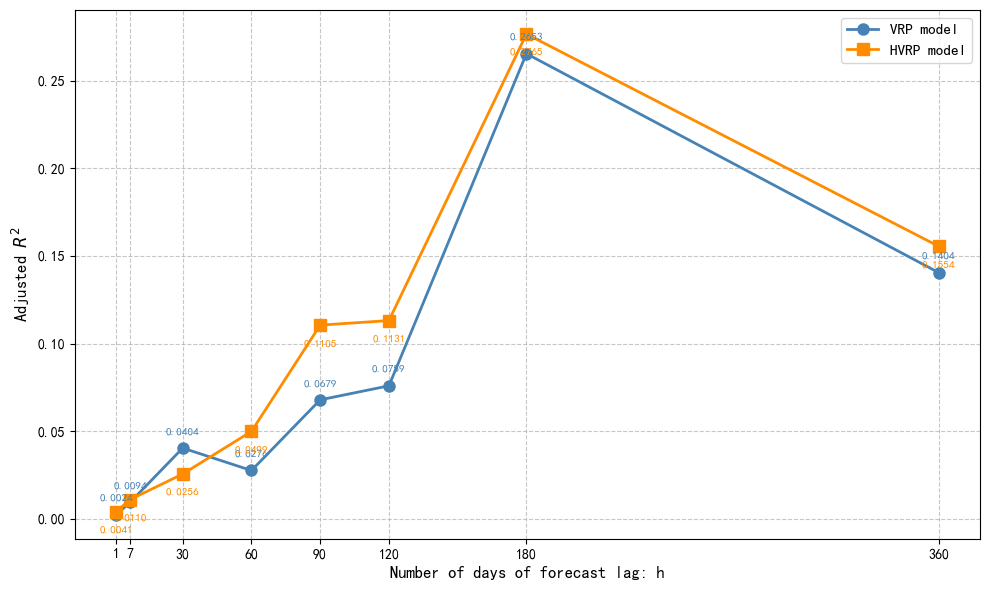
\includegraphics[width=0.9\linewidth]{eng r2.png}
    \caption{Comparison of $R^2$ Values for the Two Models}
    \label{fig:placeholder}
\end{figure}

\section{Conclusions and Outlook}
\subsection{Research Conclusions}
Based on 5-minute high-frequency return data for the Huatai-PineBridge CSI 300 ETF on the Shanghai Stock Exchange from January 2020 to October 2025, along with corresponding daily option trading data, this paper systematically examines the predictive power, term structure characteristics, and asymmetric effects of the VRP on the ETF’s returns. It also optimizes the construction of the VRP by introducing a heterogeneous autoregressive realized volatility (HARV) model. The study reaches the following main conclusions:

First, the VRP exhibits significant predictive power for the returns of the CSI 300 ETF, and this predictive power displays distinct term structure characteristics. Within the medium-term forecast window of 30 to 90 days, the VRP exhibits a positive predictive effect on returns, implying that when the implied volatility risk premium in the options market rises, the underlying ETF tends to receive higher return compensation over the medium term; whereas in the long-term forecast window of 120 days or more, the predictive direction of the VRP reverses to negative, and the significance level further increases to the 1‰ level. This conclusion remains robust in both univariate and multivariate regression models. This term structure characteristic indicates that the mechanism through which volatility risk pricing information expressed by investors in the options market influences spot returns differs fundamentally between the medium and long term: the medium term reflects risk compensation logic to a greater extent, while the long term may imply a combined effect of mean reversion and market sentiment correction.

Second, there is significant asymmetry in the predictive effects of positive and negative VRPs on returns. Decomposition results show that the positive VRP possesses stable negative predictive power for returns within long-term forecasting windows of 120 days or more, whereas the predictive power of the negative VRP declines significantly in the ultra-long-term window of 360 days, indicating that the market information contained in the VRP has largely been priced in over the ultra-long term. This finding confirms the asymmetry in the pricing mechanisms of upward and downward volatility risks in China’s CSI 300 ETF market, where the predictive information of the downward volatility risk premium decays more rapidly, providing a reference for investors’ differentiated market timing strategies.

Third, the HAR-VRP indicator, optimized using the HAR-RV model, outperforms the traditional VRP in predictive performance within a multiple regression framework. Comparative results show that after incorporating HAR-RV for volatility forecasting, the adjusted R² of the multiple regression model improved to varying degrees across all forecast horizons of 60 days and longer, with the goodness of fit peaking around the 180-day horizon. This indicates that by incorporating realized volatility information across multiple time scales—including daily, weekly, and monthly—the HAR-RV model can more accurately capture the true volatility structure of the underlying asset, thereby enhancing the predictive power of the VRP indicator for medium- to long-term returns. This finding provides new empirical evidence for optimizing the measurement of the VRP and improving asset return forecasting methods.

Fourth, implied volatility-related variables generally exhibit robust significance in long-term forecasting. Whether it is the VRP and HAR-VRP examined in this paper or the mean of implied volatility, the spread between call and put option implied volatilities, and the VIX index, all demonstrate strong predictive power in long-term forecasting windows of 120 days or more, with relatively stable levels of significance. In contrast, the call-put volume spread—a volume-based indicator—exhibits only weak predictive power in isolated medium-term windows and fails to remain effective over the long term. This comparison further confirms that the forward-looking market expectations embedded in implied volatility are the core drivers of long-term return forecasts, whereas the information contained in volume-based indicators has a shorter time horizon.


\subsection{Research Outlook}
This paper conducts a systematic empirical study on the predictive effect of the VRP on the returns of the CSI 300 ETF and makes preliminary explorations in model optimization; however, several areas warrant further investigation:

First, regarding the research on the transmission mechanism through which the VRP influences returns, the empirical analysis in this paper focuses on testing the existence, direction, and term structure of the predictive effect. The analysis of the underlying mechanisms through which the VRP affects the returns of the underlying assets is not yet sufficiently in-depth. Future research could attempt to incorporate mediating variables such as investor sentiment, market liquidity, and margin trading constraints to construct a more comprehensive framework for analyzing transmission channels, thereby further clarifying the micro-level mechanisms through which pricing information from the VRP is transmitted to the spot market.

Second, regarding the extension of volatility forecasting models, this study employs the classic HAR-RV model to forecast realized volatility. Future research could explore the HAR-RV-CJ model to further distinguish between continuous and jump volatility components, or adopt extended models such as HARQ and SHAR that account for measurement error and structural changes, to improve volatility forecasting accuracy and thereby enhance the quality of VRP construction and the effectiveness of yield forecasting.

Third, regarding the expansion of the sample and underlying assets, CSI 300 ETF options have been listed and traded for only a relatively short period. In the future, as the sample period continues to extend and market microstructure matures, it will be possible to further examine the time-varying characteristics and state-dependence of VRP’s predictive capabilities across different market cycle phases. At the same time, with the successive listing of various exchange-traded option products, such as the CSI 500 ETF options and ChiNext ETF options, conducting cross-sectional comparative studies on the VRP forecasting effects for ETFs with different market capitalization styles will also help to gain a more comprehensive understanding of the commonalities and differences in volatility risk pricing across China’s multi-tiered capital markets.

	% ==================== 参考文献区 ====================
	\newpage
	\renewcommand\refname{References} % 如果是article类，默认是“参考文献”；如果是report类，可改为 \bibname
	\addcontentsline{toc}{section}{References} % 将参考文献加入目录
	
	\begin{thebibliography}{99} % 99表示最大标号宽度
\bibitem{merton1973}
Merton, R. C. (1973). An intertemporal capital asset pricing model. \textit{Econometrica}, 41(5), 867–887.

\bibitem{andersen1998}
Andersen, T. G., \& Bollerslev, T. (1998). Answering the skeptics: Yes, standard volatility models do provide accurate forecasts. \textit{International Economic Review}, 39(4), 885–905.

\bibitem{brittenjones2000}
Britten-Jones, M., \& Neuberger, A. (2000). Option prices, implied price processes, and stochastic volatility. \textit{The Journal of Finance}, 55(2), 839–866.

\bibitem{bollerslev2009}
Bollerslev, T., Tauchen, G., \& Zhou, H. (2009). Expected stock returns and variance risk premia. \textit{The Review of Financial Studies}, 22(11), 4463–4492.

\bibitem{bollerslev2014}
Bollerslev, T., Patton, A. J., \& Quaedvlieg, R. (2014). Good volatility, bad volatility: Signed jumps and the predictability of returns. \textit{Journal of Financial Economics}, 114(3), 516–534.

\bibitem{drechsler2011}
Drechsler, I., \& Yaron, A. (2011). What’s vol got to do with it. \textit{The Review of Financial Studies}, 24(1), 1–45.

\bibitem{rapach2013}
Rapach, D. E., Strauss, J. K., \& Zhou, G. (2013). International stock return predictability: What is the role of the United States? \textit{The Journal of Finance}, 68(4), 1633–1662.

\bibitem{carr2007variancessrn}
Carr, P. P., \& Wu, L. (2007). Variance Risk Premia. \textit{SSRN Electronic Journal}. http://www.ssrn.com/abstract=577222

\bibitem{carr2009variance}
Carr, P., \& Wu, L. (2009). Variance Risk Premiums. \textit{Review of Financial Studies}, 22(3), 1311–1341. 

\bibitem{dai2020efficient}
Dai, Z., Zhou, H., Wen, F., \& He, S. (2020). Efficient predictability of stock return volatility: The role of stock market implied volatility. \textit{The North American Journal of Economics and Finance}, 52, 101174. 

\bibitem{londono2017variance}
Londono, J. M., \& Zhou, H. (2017). Variance risk premiums and the forward premium puzzle. \textit{Journal of Financial Economics}, 124(2), 415–440. 

\bibitem{bollerslev2014stock}
Bollerslev, T., Marrone, J., Xu, L., \& Zhou, H. (2014). Stock Return Predictability and Variance Risk Premia: Statistical Inference and International Evidence. \textit{Journal of Financial and Quantitative Analysis}, 49(3), 633–661.

\bibitem{timmermann2018forecasting}
Timmermann, A. (2018). Forecasting Methods in Finance. \textit{Annual Review of Financial Economics}, 10(1), 449–479.

\bibitem{huang2016modeling}
Huang, Z., Liu, H., \& Wang, T. (2016). Modeling long memory volatility using realized measures of volatility: A realized HAR GARCH model. \textit{Economic Modelling}, 52, 812–821. 

\bibitem{qiao2024variance}
Qiao, F., Xu, L., Zhang, X., \& Zhou, H. (2024). Variance risk premiums in emerging markets. \textit{Journal of Banking \& Finance}, 167, 107259.

\bibitem{carr2001volatilitytrading}
Carr, P., \& Madan, D. (2001). Towards a Theory of Volatility Trading. In E. Jouini, J. Cvitanic, \& M. Musiela (Eds.), \textit{Option Pricing, Interest Rates, and Risk Management} (pp. 458–476). Cambridge University Press, Cambridge.

\bibitem{corsi2012harmodeling}
Corsi, F., Audrino, F., \& Renò, R. (2012). HAR Modeling for Realized Volatility Forecasting. In L. Bauwens, C. Hafner, \& S. Laurent (Eds.), \textit{Handbook of Volatility Models and Their Applications} (pp. 363–382). Wiley.

\bibitem{londono_vrpworld}
Londono, J. M. (2011). The variance risk premium around the world. \textit{International Finance Discussion Papers}, No. 1035, pp. 1-55.

\bibitem{zhou_vrpreview}
Zhou, H. (2018). Variance risk premia, asset predictability puzzles, and macroeconomic uncertainty. \textit{Annual Review of Financial Economics}, 10, 481-497.

\bibitem{engle1982arch}
Engle, R. F. (1982). Autoregressive conditional heteroscedasticity with estimates of the variance of United Kingdom inflation. \textit{Econometrica}, 50(4), 987-1007.

\bibitem{hansen2010realizedgarch}
Hansen, P. R., \& Shek, H. H. (2010). Realized GARCH. CREATES Research Paper 2010-13, pp. 1-62.

\bibitem{li_longmemoryvolatility}
Li, J., Phillips, P. C. B., Shi, S., \& Yu, J. (2022). Weak identification of long memory with implications for volatility modeling. SMU Economics and Statistics Working Paper Series, No. 08-2022, pp. 1-49.

\bibitem{chenrong2009}
CHEN, R., ZHENG, Z. L. (2009). Volatility risk premium: Models and empirical evidence. \textit{Journal of Management Sciences in China}, 12(4), 112–122. (in Chinese)

\bibitem{zhenzhenlong2013}
ZHENG, Z. L., LIU, Y. S. (2013). Volatility risk premium and predictability of stock returns. \textit{Journal of Financial Research}, (10), 156–170. (in Chinese)

\bibitem{huangyizhou2016}
HUANG, Y. Z., ZHENG, Z. L. (2016). Model-free implied volatility and its information content: Evidence from CSI 300 ETF options. \textit{Journal of Financial Research}, (11), 159–174. (in Chinese)

\bibitem{chenguojin2018}
CHEN, G. J., ZHANG, R. Z., YAO, D. J. (2018). Tail risk, volatility risk premium, and stock returns. \textit{Journal of Financial Research}, (10), 112–128. (in Chinese)

\bibitem{chenrong2021}
CHEN, R., GE, J., YU, J. (2021). Volatility risk premium in China’s stock market: Empirical evidence based on ETF options. \textit{Systems Engineering — Theory & Practice}, 41(5), 1121–1138. (in Chinese)

    \end{thebibliography}
    
\end{document}

